\chapter{Pre-Processing}
\label{chap6}

\section{Motivation}
As previously discussed in Section \ref{chap2Ass}, a pre-processing step is employed to remove some of the noise introduced by the shredding and scanning process and bring the shreds to a standard form which can be used in the rest of the algorithm. To shortly re-iterate, we want to take the scanned image and return individual images for each shred, such that the shreds are correctly orientated, are all the same size and contain only white and black pixels.

The goal of the pre-processing step can be intuitively seen in Figure \ref{fig:preProc}.

\section{Segmentation and Skew}
First of all, the shreds need to be picked out from the background. In order to simplify this process, a background colour which is significantly different from both white and black needs to be chosen (in the case of Figure \ref{fig:preProc} it has an RGB value of \emph{(255,127,0)}). In order to identify the shred pixels, we can declare a threshold value $\tau$ and then say that a pixel \emph{p} belongs to the background if \footnote{here we assume that $p[0]$, $p[1]$ and $p[2]$ correspond to the red, green and blue values of pixel $p$} \[ |p[0] - background[0]| + |p[1] - background[1]| + |p[2] - background[2]| \leq \tau \] As reported in \cite{P26}, automatically setting a $\tau$ value is not easy, as the optimal value depends on the noise level in the scanned image. We just choose a value empirically, by running a few tests on the input data.

\begin{figure}[H]
        \setlength{\fboxsep}{-0.1cm}
        \centering
        \begin{subfigure}[b]{\textwidth}
                \centering
                
\includegraphics[width=\textwidth]{scrambled}
                \caption{Scanned image given as input.}
        \end{subfigure}
        \begin{subfigure}[b]{\textwidth}
                \centering
                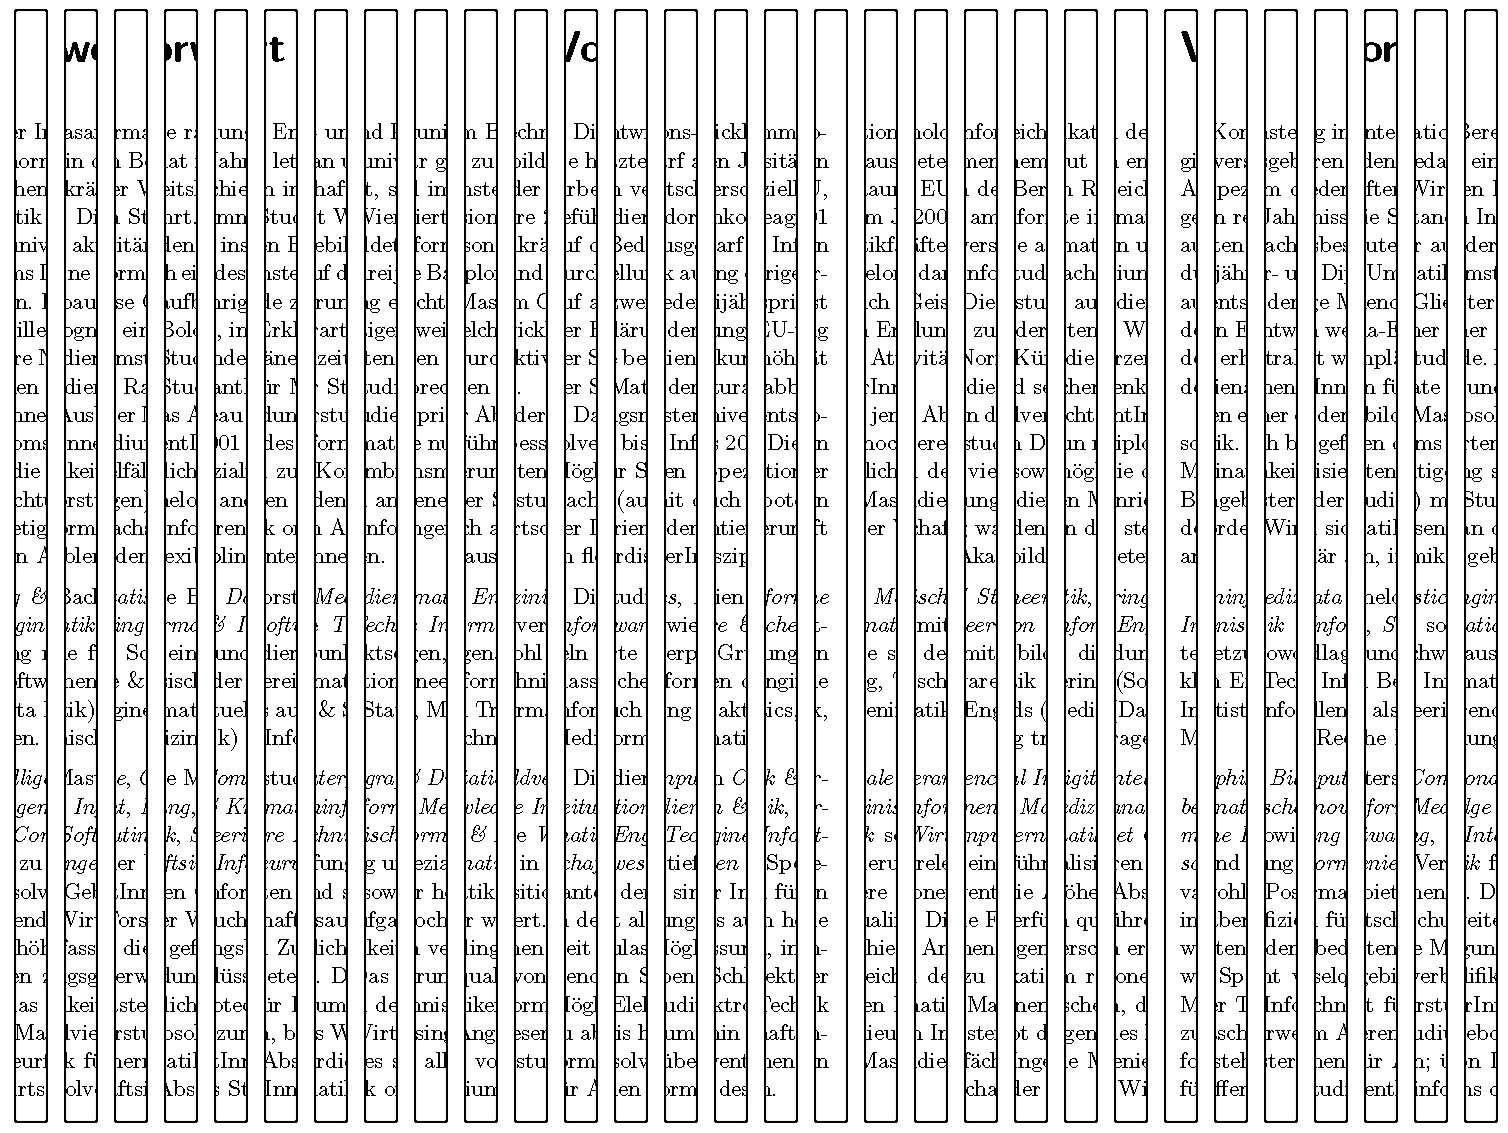
\includegraphics[width=\textwidth]{idealShreds}
        \caption{Individual \emph{ideal shred} images outputted.}
        \end{subfigure}
        \caption{Desired input and output of the Pre-Processing function. }
        \label{fig:preProc}
\end{figure}

After the potential shred pixels are identified, we next group them into continuous blobs. This is done by assigning an initial set to each pixel and then checking each pixel's 8 neighbours. If a neighbouring pixel is found, then the two have their sets merged. After these blobs are identified, the groups smaller than 100 pixels are discarded as noise (unless we are working with micro-shredders, it's quite unlikely a shred will have a size of less than 10x10 pixels). The remaining blobs of pixels are our shreds.

The next step is to fix the skew of the shreds, so that their edges become placed either vertically or horizontally. First the corners of the shreds are identified as the topmost, bottommost, leftmost and rightmost points in each shred. We then identify the edges running between these points, using the criteria that edge pixels are neighbours with at least one background pixel. Once the edges are known, we pick one of the long edges and, for each pixel on that edge, we calculate how much the shred would have to be rotated such that the edge pixel would be placed on a vertical line containing both its corner pixels (see Figure \ref{fig:skew}). Finally, we choose the median of all the calculated angles as the final angle by which the shred will be rotated. 

\begin{figure}[h]
    \centering
    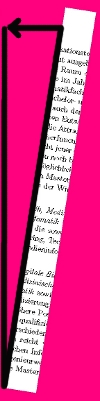
\includegraphics[width=0.17\textwidth]{skew}
    \caption{The triangle showing how much a certain pixel would need to be moved to be placed on the vertical line (in this case, about 10 degrees).}
    \label{fig:skew}
\end{figure}

Once the rotation is known, we can proceed with the segmentation. First a rough bounding box is made around each shred, thus allowing a different image to be created for every shred. Each of these images is then rotated by the required amount as to fix the skew of the shreds. The next step is to go over each pixel once more and record the height and width of each shred for every row and every column in the shred. The median height and median width over all these values are then taken as the final dimensions of the shreds and each image is cropped to that size. 

We now have individual images for each shred, which are all of the same size and which are either correctly oriented or rotated by 180 degrees.

\section{Up/down orientation detection}
This is the final step which will make sure that all shreds are ``the right way up". Here we want to identify the shreds which are upside down and rotate them by 180 degrees.

We employ a simple method based on row detection. The goal is to detect both the ``inner" and ``outer" rows on each shred (see Figure \ref{fig:rows}). The outer rows are defined as those y coordinates in which a transition is made between a row that contains no black pixels and a row that contains at least 1 black pixel. The resulting ``outer rows" are then filtered such that only those wider than a minimum threshold are kept, since a row that is only 1 or 2 pixels wide is quite likely spurious. We then want to find an ``inner row" inside each remaining ``outer row". The inner rows are defined as the y coordinates exhibiting the greatest difference between the sum of black pixels in two consecutive rows. So when we detect the greatest increase in number of black pixels between 2 consecutive rows, we call this the upper limit of the inner row, and when we detect the greatest decrease we call it the lower limit of the inner row.

\begin{figure}[h]
    \centering
    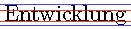
\includegraphics[width=\textwidth]{innerOuterRows}
    \caption{Red lines delimitate the inner row, blue lines delimitate the outer row.}
    \label{fig:rows}
\end{figure}

After this is done, we count the number of black pixels in the ``upper region" and ``lower region", which are the areas between the inner and outer rows placed below and above each shred (see Figure \ref{fig:regions}). We then sum up all of these numbers and predict that a shred will have more black pixels in the ``upper regions".

\begin{figure}[h]
    \centering
    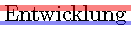
\includegraphics[width=\textwidth]{EntRow}
    \caption{The upper region is in red and the lower one in blue. For Roman script, the upper regions will generally contain more black pixels.}
    \label{fig:regions}
\end{figure}

This simple orientation detection method does surprisingly well\footnote{This experiment uses ideal shreds. Preliminary tests indicate that the method works similarly on real scanned shreds, as long as the skew correction function produces results within 1-2 degrees of vertical.}, as can be seen in Figure \ref{fig:orientation}.

\begin{figure}[h]
    \centering
    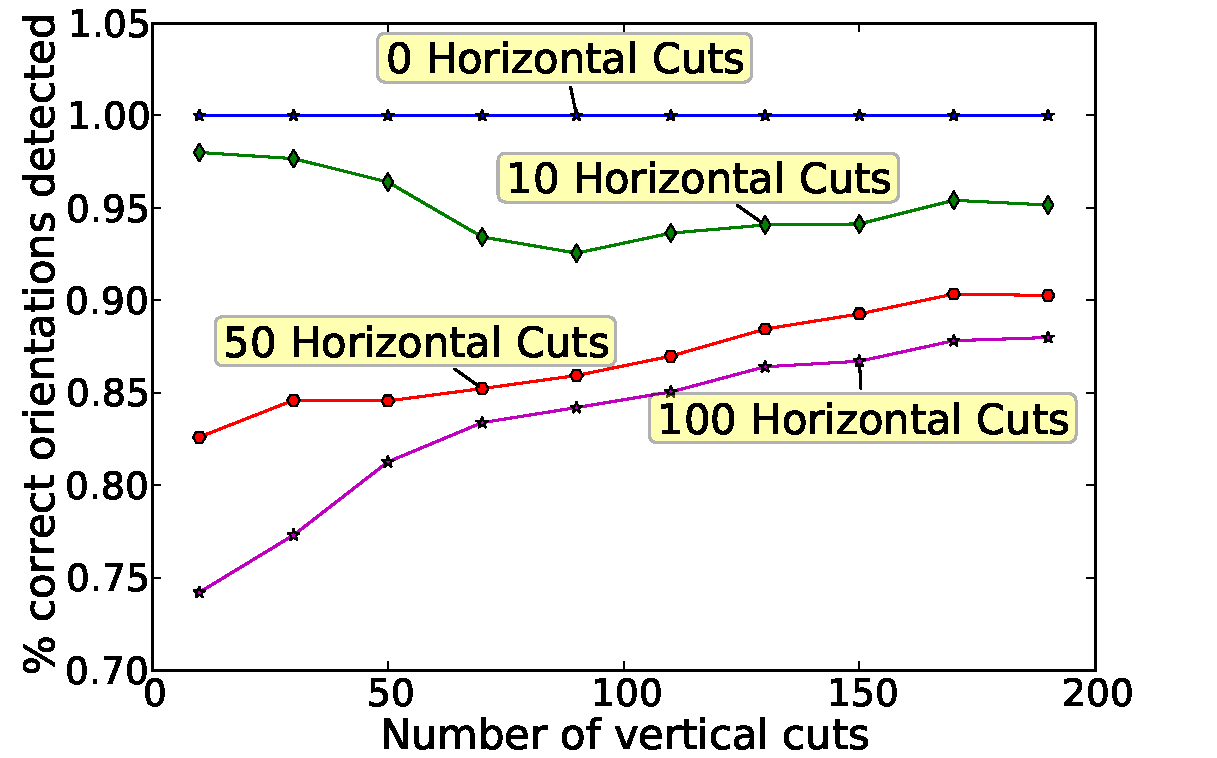
\includegraphics[width=\textwidth]{orientation.pdf}
    \caption{The proportion of correctly oriented shreds.}
    \label{fig:orientation}
\end{figure}

As can be seen, the results are perfect for strip-cut documents (i.e. 0 horizontal cuts) and steadily degrade as we introduce more horizontal cuts. This happens because horizontal cuts reduce the number of rows printed on each shred and therefore make the system more vulnerable to noise. It is worth noting that in the lower two curves, the odd behaviour of the performance getting better as the number of vertical cuts increases is caused by completely white pieces. Completely white pieces are declared as being always correctly oriented and, when both the number of vertical and horizontal cuts are high, there are a lot of completely white pieces. For the lower two curves, increasing the number of vertical cuts increases the number of white pieces faster than the added noise can degrade the performance, so the overall proportion of correctly predicted orientations increases.

In conclusion, this simple orientation detection method works quite well as long as the number of horizontal cuts is small. For more robust solutions that handle cross-cut documents better or that also work on non-Roman script, one of the methods discussed in Section \ref{chap3PP} could be implemented.

\section{Limitations}

There are two main limitations of the pre-processing method described above which together were severe enough to prevent the system from working on real scanned shreds.

The first problem comes from the skew correction. It seems that any rotation\footnote{Document rotation was done using both the Python Imaging Library \cite{P52} and the ImageMagick ``convert" command \cite{P53}. No qualitative difference was observed between the two methods.} above 1 or 2 degrees can significantly distort the source image (see Figure \ref{fig:skewProb}). As shown in Section \ref{chap4Rob}, this type of noise will deteriorate the performance of the probabilistic model. The problem here is exacerbated since not all shreds will be rotated the same amount and therefore some shreds will be distorted more than other. This non-uniformity further confuses the scoring function.

\begin{figure}[h]
        \setlength{\fboxsep}{-0.1cm}
        \centering
                \begin{subfigure}[t]{0.47\textwidth}
                        \centering
                        \fbox{ 
                        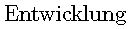
\includegraphics[width=\textwidth]{EntOrig}
                        }
                        \caption{Original document.}
                \end{subfigure}
                \begin{subfigure}[t]{0.47\textwidth}
                        \centering
                        \fbox{ 
                        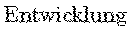
\includegraphics[width=\textwidth]{EntRot}
                        }
                        \caption{Document rotated by 10 degrees.}
                \end{subfigure}
    \caption{The noise introduced by rotating a document and recasting it to binary data.}
    \label{fig:skewProb}
\end{figure}

The second problem is caused by the ``curviness" of the strips which was briefly discussed in Section \ref{chap3PP}. While at a casual glance the original scanned strips appear to be straight, after pre-processing them it becomes clear they are actually curvy (see Figure \ref{fig:curvy}). This is a big problem for our scoring function, since it only looks at a thin context on the margin of the shred, and this is exactly the area affected by this issue.

\begin{figure}[h]
    \vspace{1em}
    \centering
    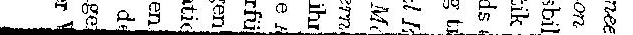
\includegraphics[width=\textwidth]{curved}
    \caption{A section of a real processed shred. The curviness causes the segmentation to fail and therefore makes part of the margin completely black. This seriously affects the performance of the scoring function.}
    \label{fig:curvy}
\end{figure}

One solution for the above problems would be to increase the complexity of the methods employed by the pre-processing function. The rotation noise could be mitigated by doing the rotation at a high resolution and then downsampling the image. Specific smoothing operators could also be employed as to minimize the difference between shreds rotated by different amounts. The issue with curvy strips could could be mitigated by the method suggested in \cite{P26}, namely fitting a polynomial in order to find the true edges. Afterwards the shred could be forced back into a rectangle, though the noise introduced by this modification might further complicate the task.

Alternatively, another solution would be to improve the scanning process as to remove these problems before the pre-processing step. This approach is taken in \cite{P51}, where the authors find that carefully securing the strips to a rigid background can eliminate both their tendency to curve and the need to correct their skew by more than a couple degrees.
